%
% 4-schnell.tex
%
% (c) 2022 Prof Dr Andreas Müller, OST Ostschweizer Fachhochschule
%
\section{Schnelle Algorithmen für die Fourier-Transformation
\label{buch:diskret:section:schnell}}
\kopfrechts{Schnelle Algorithmen}
Die Berechnung Fourier-Transformierten $\hat{f}=\mathscr{F}_nf$ eines
$n$-dimensionalen Vektors $f$ als Produkt einer $n\times n$-Matrix mit
einem Vektor benötigt $n^2$ Multiplikationen und $n(n-1)$ Additionen,
also $O(n^2)$ Operationen.
Verdoppelung der Vektorlänge führt zu einer Vervierfachung der Rechenzeit.
Für zweidimensionale Anwendungen, wie sie in der Bildverarbeitung
benötig werden, ergibt sich sogar ein Faktor 16.
Die Rechenzeit limitiert die Nützlichkeit der Fourier-Transformation
beträchtlich.
In diesem Abschnitt soll gezeigt werden, wie die in
Abschnitt~\ref{buch:diskret:section:vandermonde} hergeleitete
Faktorisierung der Vandermonde-Matrix ermöglicht, die Fourier-Transformation
in $O(n\log n)$ statt $O(n^2)$ Operationen berechnet werden kann.

%
% Primfaktorisierung von $n$
%
\subsection{Primfaktorisierung von $n$
\label{buch:diskret:schnell:subsection:primfaktorisierung}}
Der Fundamentalsatz der Arithmetik besagt, dass jede natürlich Zahl $n$
eine bis auf die Reihenfolge der Faktoren eindeutige Zerlegung in
Primfaktoren
\begin{equation}
n = p_1^{n_1} p_2^{n_2} \cdots p_k^{n_k}
\label{buch:diskret:schnell:eqn:pfakt}
\end{equation}
hat.
Die Faktorisierung kann wie folgt rekursiv gefunden werden.
Sei $p_1,p_2,p_3,\dots$ die aufsteigende Folge aller Primzahlen, die
$\le \sqrt{n}$ sind.
Jetzt werden der Reihe nach alle Primzahlen $p_l$ daraufhin getestet,
ob sie $n$ teilen.
Wenn kein Teiler gefunden wird, dann ist $n$ eine Primzahl und kann
nicht weiter faktorisiert werden.
Ist $p_l\mid n$ ein Teiler, dann ist $m=n/p_l$ eine natürlich Zahl
und die Zahl $n$ kann als $n=p_l\cdot m$ faktorisiert werden.

Aus der Primfaktorisierung~\eqref{buch:diskret:schnell:eqn:pfakt}
von $n$ lasen sich alle möglichen Faktorisierungen ablesen.
Zwei Faktor $m'$ und $m''$ haben ihre eigenen Faktorzerlegungen
\[
m'= p_1^{n_1'}p_2^{n_2'}\cdots p_k^{n_k'}
\qquad\text{und}\qquad
m''= p_1^{n_1''}p_2^{n_2''}\cdots p_k^{n_k''}.
\]
Damit $m'\cdot m''=n$ gilt, müssen für die Exponenten die Gleichungen
\[
n_1=n_1'+n_1'',\quad
n_2=n_2'+n_2'',\quad\dots\quad
n_k=n_k'+n_k''
\]
gelten.
Da alle $n_i'$ und $n_i''$ natürliche Zahlen sein müssen, muss
\[
0\le n_i'\le n_i
\]
für alle $i=1,\dots,k$ sein.
Es gibt daher
\[
(n_1+1)(n_2+1)\dots(n_k+1)
\]
Faktorisierungen der Form
\[
n
=
\underbrace{
p_1^{n_1'}p_2^{n_2'}\cdots p_k^{n_k'}
}_{\displaystyle m'}
\underbrace{
p_1^{n_1-n_1'}p_2^{n_2-n_2'}\cdots p_k^{n_k-n_k'}
}_{\displaystyle m''}
\]

Für jede mögliche Faktorisierung $n=m'\cdot m''$ gibt es nach
Satz~\ref{buch:diskret:vandermonde:satz:fourierfaktorisierung}
der Fourier-Transformation $\mathscr{F}$ in zwei Faktoren
\[
\mathscr{F}_n
=
%\frac{1}{m''}
A(m',m'',\omega) (\mathscr{F}_{m'} \otimes I_{m''})
\]
mit $\omega=e^{-2\pi i/n}$.

%
% Zerlegung in drei Faktoren
%
\subsection{Zerlegung in drei Faktoren
\label{buch:diskret:schnell:subsection:dreifaktoren}}
\begin{figure}
\centering
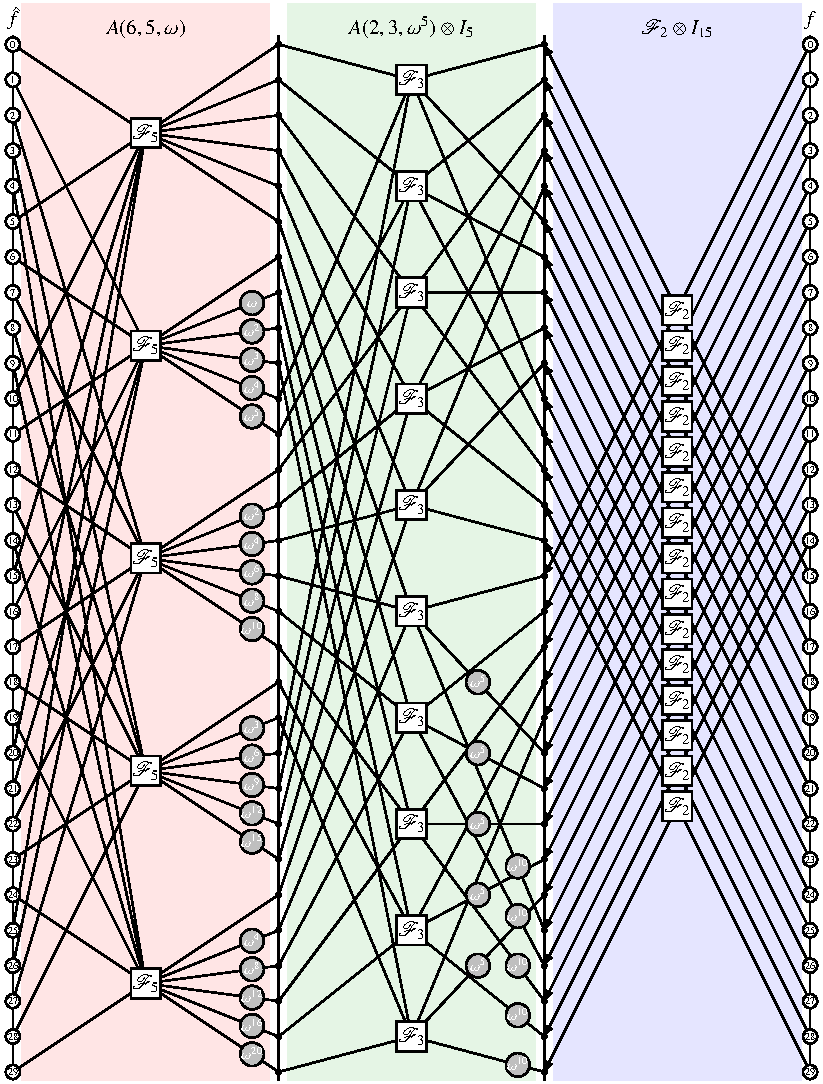
\includegraphics{chapters/060-diskret/images/f30.pdf}
\caption{Faktorisierung der Fourier-Transformation
$\mathscr{F}_{30}$ in die Faktoren
$\mathscr{F}_{30}
=
A(6,5,\omega)
\cdot
(A(2,3,\omega^5)\otimes I_5)
\cdot
(F(2,3,\omega^5)\otimes I_5)
=
A(5,6,\omega)
\cdot
(A(3,2,\omega^5)\otimes I_5)
\cdot
(\mathscr{F}_2\otimes I_{15})
$.
\label{buch:diskret:faktorisierung:fig:f30}}
\end{figure}
Wir betrachten eine Faktorisierung von $n=n_1n_2n_3$ in drei Faktoren
und setzen $\omega = e^{-2i\pi/n}$.
Indem wir $p=n_1n_2$ und $q=n_3$ setzen, können wir die Fourier-Transformation
als
\begin{equation}
\mathscr{F}_n
=
A(p,q,\omega)
=
A(p,q,\omega) \mathscr{F}_p\otimes I_q
=
A(n_1n_2,n_3,\omega) \cdot \mathscr{F}_{n_1n_2}\otimes I_{n_3}
\label{buch:diskret:schnell:eqn:dreifaktoren1}
\end{equation}
faktorisieren.
Der Faktor $\mathscr{F}_{n_1n_2}$ kann wieder faktorisiert werden
als
\begin{align*}
\mathscr{F}_{n_1n_2}
&=
A(n_1,n_2,\omega^{n_3}) \cdot \mathscr{F}_{n_1}\otimes I_{n_2}.
\intertext{Zusammen mit~\eqref{buch:diskret:schnell:eqn:dreifaktoren1}}
\mathscr{F}_n
&=
A(n_1n_2,n_3,\omega)
\cdot
(A(n_1,n_2,\omega^{n_3})\otimes I_{n_3})
\cdot
\mathscr{F}_{n_1}\otimes I_{n_2n_3}.
\end{align*}
Abbildung~\ref{buch:diskret:faktorisierung:fig:f30} zeigt die Situation
für $n=30=2\cdot 3\cdot 5$ mit $n_1=2$, $n_2=3$ und $n_3=5$.

%
% Faktorzerlegung der Fourier-Transformation
%
\subsection{Volle Faktorzerlegung der Fourier-Transformation
\label{buch:diskret:schnell:subsection:fourierfaktorisierung}}
Sei jetzt $n=n_1n_2\dots n_k$ eine Faktorisierung von $n$.
Wir bezeichnen mit $n_i'$ das Produkt der Faktoren, die nach dem Faktor
$i$ stehen, also
\[
n_i'
= 
n_{i+1}\dots n_k.
\]
Speziell ist $n_{k-1}'=n_k$.
Daraus leitet man ab, dass
\[
n
=
n_1n_1'
=
n_1n_2n_2'
=
\ldots
=
n_1\dots n_ln_l'
=
\dots = n_1\dots n_{k-1}n_k
\]
gilt.
Ausserdem folgt
\[
n_l'
=
n_{l+1}n_{l+1}'
\]
für alle $l=1,\dots,k-1$.

Die Fourier-Transformation $\mathscr{F}_n$ kann zerlegt werden in die
Faktor $A(n_1,n_1',\omega)$ und $F(n_1,n_1',\omega)$.
Den zweiten Faktor können wir als das Kronecker-Produkt
\[
F(n_1,n_1',\omega)
=
\mathscr{F}_{n_1} \otimes I_{n_1'}
\]
schreiben.
Da $n_1'=n_2n_2'$, kann auch $\mathscr{F}_{n_1'}$ analog zerlegt werden
als
\[
\mathscr{F}_{n_1'}
=
A(n_2,n_2',\omega^{n_1}) (\mathscr{F}_{n_2}\otimes I_{n_2'}).
\]
Das Kronecker-Produkt von rechts mit $I_{n_1}$ ergibt
\[
\mathscr{F}_{n_1'}\otimes I_{n_1}
=
(A(n_2,n_2',\omega)\otimes I_{n_1})
(\mathscr{F}_{n_2}\otimes I_{n_1n_2}).
\]
Durch Wiederholung dieser Faktorisierung ergibt sich daher die
vollständige Faktorisierung
\begin{equation}
\mathscr{F}_n
=
A(n_1,n_1',\omega)
\cdot
(A(n_2,n_2',\omega^{n_1})\otimes I_{n_1})
\cdot
(A(n_3,n_3',\omega^{n_1n_2})\otimes I_{n_1n_2})
\cdot
\ldots
\cdot
(\mathscr{F}_{n_k}\otimes I_{n_1\dots n_{k-1}})
\label{buch:diskret:schnell:eqn:faktorisierung}
\end{equation}
von $\mathscr{F}_n$.

Die Faktorisierung~\eqref{buch:diskret:schnell:eqn:faktorisierung}
ermöglich jetzt eine schnellere Berechnung der Fourier-Transformation.
Jeder der Matrizen $A(p,q,\omega^l)$ enthält in jeder Zeile genau
$p$ von $0$ verschiedene Einträge.
Das Produkt einer solchen Matrix mit einem Vektor kann daher in 
$O(pn)$ Operationen berechnet werden.
Der Gesamtaufwand zur Berechnung von $\mathscr{F}_nf$ mit Hilfe
der Faktorisierung ist daher 
\(
O((n_1+n_2+\dots+n_k)n)
\)
statt $O(n^2)$.

\begin{figure}
\centering
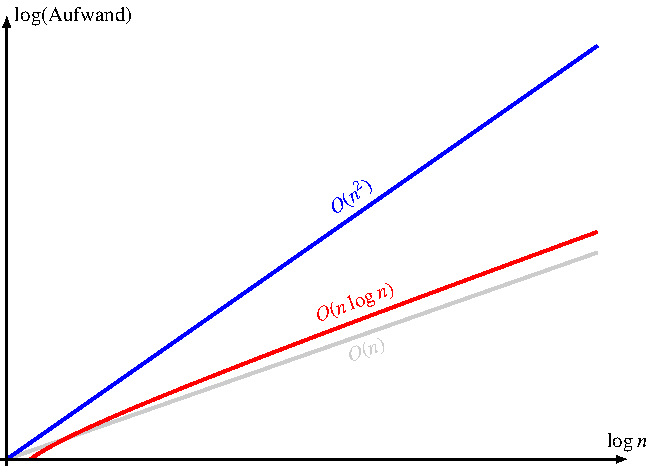
\includegraphics{chapters/060-diskret/images/log.pdf}
\caption{Vergleich des Rechenaufwandes für die Fourier-Transformation
$\mathscr{F}_n$ mit der direkten Matrixmultiplikation (blau) und
mit Hilfe der 
Faktorisierung~\eqref{buch:diskret:schnell:eqn:faktorisierung}
(rot).
\label{buch:diskret:schnell:fig:log}}
\end{figure}%

Der Rechenaufwand kann noch etwas klarer abgeschätzt werden, wenn 
die Grösse der Faktoren der 
Faktorisierung~\eqref{buch:diskret:schnell:eqn:faktorisierung}
abgeschätzt werden kann.

\begin{satz}
\label{buch:diskret:schnell:satz:aufwand}
Ist $n=n_1n_2\cdot\ldots\cdot n_k$ eine Faktorisierung von $n$
mit $n_i\le b$ für alle $i$, dann lässt sich die Fourier-Transformation
$\mathscr{F}_n$ mit einem Aufwand höchstens $O(n\log_b n)$ berechnen.
\end{satz}

\begin{proof}[Beweis]
Weil $n_i\le b$ gilt, folgt
\[
\log_b n=\log_bn_1+ \ldots +\log_b n_k
\le 
k\log_b b
=
k.
\]
Andererseits sind alle Faktoren $n_i\ge 2$, so dass auch $k\le \log_2 n$
sein muss.
Es folgt, dass $k=O(\log n)$.

Für die Berechnung des Aufwandes wird die Summe der Faktoren nötig,
sie kann abgeschätzt werden durch
\[
n_1+\ldots+n_k
\le
kb.
\]
Der Aufwand ist daher
\(
O(n(n_1+\ldots+n_k))
\le
O(nbk)
=
O(n\log_b n)
\).
\end{proof}

%
% Der Fall n=2^r
%
\subsection{Der Fall $n=2^r$
\label{buch:diskret:schnell:subsection:n=2r}}
Satz~\ref{buch:diskret:schnell:satz:aufwand} zeigt, dass 
die Faktorisierung zu einer schnellen Berechnung der Fourier-Transformation
ermöglicht, die umso effizienter ist, je kleiner die Faktoren $n_i$
sind und umso mehr Faktoren die Faktorisierung hat.
Der kleinste mögliche Faktor ist $n_i=2$, dies bedeutet, dass $n=2^r$
eine Zweierpotenz sein muss.

\begin{figure}
\centering
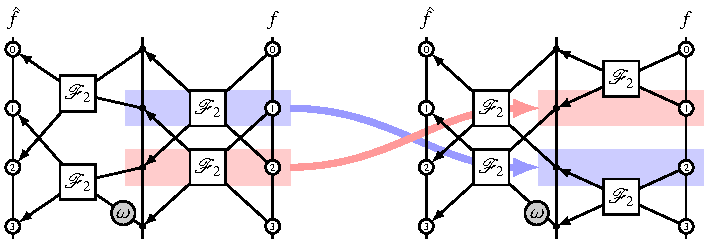
\includegraphics{chapters/060-diskret/images/f4.pdf}
\caption{Faktorisierung der Fourier-Transformation $\mathscr{F}_2
= A(2,2,\omega) (\mathscr{2}\otimes I_2)$
\label{buch:diskret:schnell:fig:f4}}
\end{figure}%
\begin{figure}
\centering
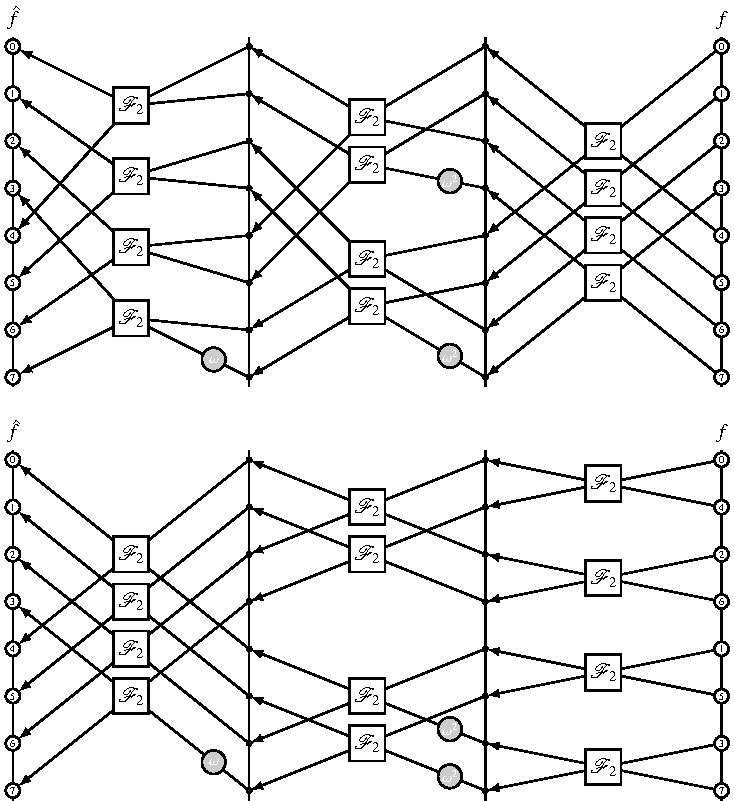
\includegraphics{chapters/060-diskret/images/f8.pdf}
\caption{Faktorisierung der Fourier-Transformation $\mathscr{F}_8$
mit Hilfe der Primfaktorisierung $8=2^3$.
Durch Umordnung der Komponenten des Vektors $f$ im unteren Schema
wird der Datenfluss übersichtlicher.
\label{buch:diskret:schnell:fig:f8}}
\end{figure}%
\begin{figure}
\centering
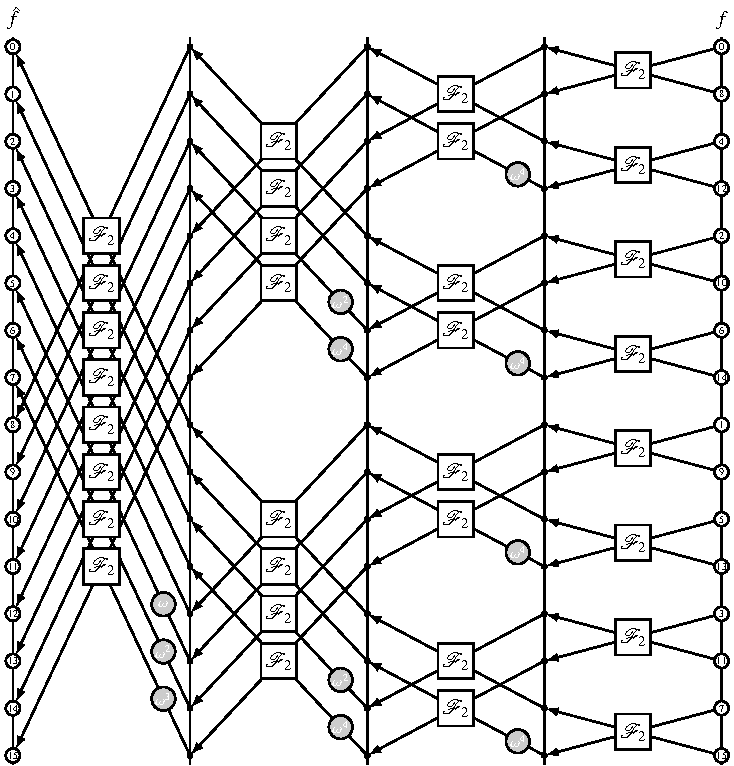
\includegraphics{chapters/060-diskret/images/f16.pdf}
\caption{Faktorisierung der Fourier-Transformation $\mathscr{F}_{16}$
mit Hilfe der Primfaktorisierung $16=2^4$.
Für den Vektor $f$ wird die Reihenfolge der Komponenten verwendet,
in der die Bitreihenfolge in den Indizes umgekehrt worden ist.
\label{buch:diskret:schnell:fig:f16}}
\end{figure}%

Abbildung~\ref{buch:diskret:schnell:fig:f4} zeigt die Faktorisierung
der Fourier-Transformation $\mathscr{F}_4$ in die zwei Faktoren
$A(2,2,\omega)$ und $\mathscr{F}_2\otimes I_2$.
Durch Umordnung der der zweiten und dritten Elemente im Vektor $f$
lässt sich eine etwas gleichmässigere Darstellung erreichen.

%
% Bitumkehr
%
\subsubsection{Bitumkehr}
Die Matrix $A(2,2^{n-1},\omega)$ kann so umgeordnet werden, dass 
sie aus $2\times 2$-Blöcken besteht, die bis auf Spaltenmultiplikationen
mit Potenzen von $\omega$ Fourier-Transformationen $\mathscr{F}_2$ sind.
Dazu müssen die Zeilen $i$ und $i+2^{n-1}$ unmittelbar nacheinander
stehen.
Numeriert man die Zeilen mit den Zahlen $0,\dots,2^n$, dann ist die
Umordnung gleichbedeutend damit, dass das erste Bit der Zeilennummer
zum letzten Bit werden muss.
Daher ist es nicht überraschend, dass eine Umordnung der Komponenten
von $f$ basierend auf der Zweiersystemdarstellung des Index zu einer
einfacheren Darstellung der Zerlegung führt.

\begin{definition}
Die {\em Bitumkehr} $\beta_k(i)$ einer Zahl $i\in\mathbb{N}$ ist
die Zahl, die sich ergibt, wenn man die Zahl $i$ als $k$-stellige
Zweiersystemzahl schreibt, nötigenfalls mit führenden Nullen,  und
dann die Reihenfolge der Ziffern umkehrt.
\end{definition}

\begin{beispiel}
Für die Zahlen $i=0,\dots,15$  ist die Bitumkehr $\beta_4(i)$ durch
die Tabelle~\ref{buch:diskret:schnell:table:bitumkehr} gegeben.
\end{beispiel}

\begin{table}
\centering
\begin{tabular}{|r|r|r|r||r|r|r|r|}
\hline
\multicolumn{2}{|c|}{$i$}&
\multicolumn{2}{|c||}{$\beta(i)$}&
\multicolumn{2}{|c|}{$\beta(i)$}&
\multicolumn{2}{|c|}{$i$}
\\
\hline
0&$\texttt{0000}_2$&$\texttt{0000}_2$& 0& 8&$\texttt{1000}_2$&$\texttt{0001}_2$& 1\\
1&$\texttt{0001}_2$&$\texttt{1000}_2$& 8& 9&$\texttt{1001}_2$&$\texttt{1001}_2$& 9\\
2&$\texttt{0010}_2$&$\texttt{0100}_2$& 4&10&$\texttt{1010}_2$&$\texttt{0101}_2$&10\\
3&$\texttt{0011}_2$&$\texttt{1100}_2$&12&11&$\texttt{1011}_2$&$\texttt{1101}_2$&13\\
4&$\texttt{0100}_2$&$\texttt{0010}_2$& 2&12&$\texttt{1100}_2$&$\texttt{0011}_2$&12\\
5&$\texttt{0101}_2$&$\texttt{1010}_2$&10&13&$\texttt{1101}_2$&$\texttt{1011}_2$&11\\
6&$\texttt{0110}_2$&$\texttt{0110}_2$& 6&14&$\texttt{1110}_2$&$\texttt{0111}_2$& 7\\
7&$\texttt{0111}_2$&$\texttt{1110}_2$&14&15&$\texttt{1111}_2$&$\texttt{1111}_2$&15\\
\hline
\end{tabular}
\caption{Bitumkehr $\beta_4(i)$ für die Zahlen $i=0,\dots,15$, betrachtet
als vierstellige Binärzahlen.
\label{buch:diskret:schnell:table:bitumkehr}}
\end{table}

Die Abbildungen 
\ref{buch:diskret:schnell:fig:f8}
und
\ref{buch:diskret:schnell:fig:f16}
zeigen den Datenfluss in der Faktorisierung der Fourier-Transformationen
$\mathscr{F}_8$ und $\mathscr{F}_{16}$.


